
\chapter{Foundations for inference}
\label{foundationsForInference}

Statistical inference is concerned primarily with understanding the quality of parameter estimates. For example, a classic inferential question is, ``How sure are we that the estimated mean, $\bar{x}$, is near the true population mean, $\mu$?'' While the equations and details change depending on the setting, the foundations for inference are the same throughout all of statistics. We introduce the common themes in Sections~\ref{CLTInformalSection}-\ref{hypothesisTesting} by discussing inference about the population proportion, $p$. Understanding this chapter will make the rest of this book, and indeed the rest of statistics, seem much more familiar.

Throughout the next few sections, we'll rely on a recurring context: the proportion of pine trees infected with mountain pine beetles. Mountain pine beetles are native to the area, but they can still do extensive damage to forests. In the past, the mountain pine beetle was held back due to hard freezes in winter. Typically a few nights of -40\degree F (same as -40\degree C!) weather kill most of the beetles and prevent them from reaching epidemic proportions. However, due to global warming, the beetles are less frequently killed by cold weather, and they have been doing severe damage to what would otherwise be healthy forests in both the United States and Canada as hard freezes become more and more rare.


%__________________
\section{Central Limit Theorem, an informal introduction}
\label{CLTInformalSection}

\Comment{Search for bad references below, which will be empty: \ref{}.}

\index{Central Limit Theorem|(}
\index{point estimate|(}

An owner of a large property in Colorado took a simple random sample of 250 mature pine trees and found that 35 have been damaged by mountain pine beetles.\footnote{While the data for this particular example are hypothetical, such a context is realistic.} The mature pine trees on the property consist of the population that the owner seeks to better understand through her sample data.

The sample proportion $\hat{p} = 35 / 250 = 0.14$ is called a \term{point estimate} of the population proportion. As we learned in Chapter~\ref{}, the sample proportion isn't perfect. It will not be exactly equal to the population proportion. However, it will tend to be close. Additionally, the larger the sample we take, the closer it will tend to be.

Figure~\ref{PineBeetleConverge} summarizes the \hiddenterm{running sample proportion} of the sample of 250 trees. As we can see, initially, the estimate was very volatile. However, as the sample became larger, it began to stabilize. The tendency of a sample proportion to become more stable as we collect more data is a property of the \term{Law of the Large Numbers}, which we first encountered in Chapter~\ref{probability}.

\begin{figure}
\centering
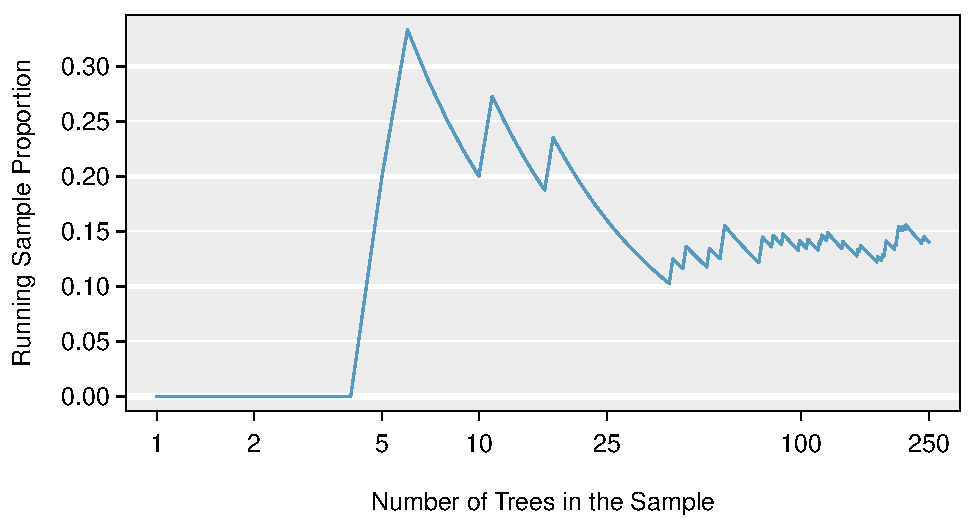
\includegraphics[width=0.85\textwidth]{05/figures/PineBeetle/PineBeetleConverge}
\caption{Running sample proportion for the pine tree sample.}
\label{PineBeetleConverge}
\end{figure}

We also learned a couple of very important details about the sample proportion in Section~\ref{distributionphat}:
\begin{enumerate}
\setlength{\itemsep}{0mm}
\item The variability of the sample proportion can be described by its standard deviation:
\begin{align*}
\sigma_{\hat{p}} = \sqrt{\frac{p(1-p)}{n}}
\end{align*}
\item The distribution of $\hat{p}$ tends to be nearly normal when we have
\begin{align*}
np &\geq 10
	& n(1-p) &\geq 10
\end{align*}
where $p$ is the population proportion and $n$ is the sample size.
\end{enumerate}
It turns out that the second characteristic is the result of a profoundly important theorem in statistics.

\begin{termBox}{\tBoxTitle{Central Limit Theorem, informal description}
Suppose we collect many independent numerical measurements. Then sample mean will tend to follow a normal distribution, \emph{even if the original data do not follow the normal distribution}.\index{Central Limit Theorem}\vspace{3mm}

We will see a more formal description of the Central Limit Theorem in the context of the sample mean in Chapter~\ref{inferenceForNumericalData}.}
\end{termBox}

A natural question is, what does this have to do with sample proportions? In fact, a lot! A sample proportion can be written down as a sample mean. For example, suppose we have 3 successes in 10 trials. If we label each of the 3 success as a 1 and each of the 7 failures as a 0, then the sample proportion is the same as the sample mean:
\begin{align*}
\hat{p}
	= \frac{1 + 0 + 0 + 1 + 1 + 0 + 0 + 0 + 0 + 0}{10}
	= \frac{3}{10}
	= 0.3
\end{align*}
That is, the sample proportion is governed by the Central Limit Theorem, and the Central Limit Theorem is what ties much of the statistical theory we will see together.

\begin{example}{Consider again the sample proportion of trees damaged by mountain pine beetles, which was 0.14 based on a sample of 250 mature pine trees. Explain how this sample proportion can be summarized as a sample mean.}
There were 35 trees identified with pine beetle damage out of the 250 trees. Label each of these trees with a 1 and the other 215 trees with a 0. Then when we take the mean of these 1's and 0's, we will get the sample proportion:
\begin{align*}
\hat{p}
	= \frac{0 + 0 + 0 + 0 + 1 + 1 + 0 + \cdots + 0 + 0}{250}
	= \frac{35}{250}
	= 0.14
\end{align*}
\end{example}

\index{point estimate|)}
\index{standard error|(}

While we will continue to focus on the sample proportion in much of this chapter, we will see a variety of estimates in Section~\ref{} where the Central Limit Theorem applies.

\index{Central Limit Theorem|)}

\begin{tipBox}{\tipBoxTitle{Three important facts}
So far, there are really three key ideas that are important:
\begin{enumerate}
\setlength{\itemsep}{0mm}
\item Point estimates from samples can be used to estimate population parameters. For example, we can use the sample proportion to estimate the true population proportion.
\item Estimates aren't perfect, and they have inherent variability. For instance, if we took two different samples and computed sample proportions based on each, they wouldn't be exactly equal.
\item When $np \geq 10$ and $n(1-p) \geq 10$, the sample proportion closely follows a normal distribution centered at $p$.
\end{enumerate}}
\end{tipBox}



%__________________
\section{Standard error and confidence intervals}

\index{confidence interval|(}
\index{confidence interval!interpretation|(}

A point estimate provides a single plausible value for a parameter. However, a point estimate is rarely perfect; usually there is some error in the estimate. Instead of supplying just a point estimate of a parameter, a next logical step would be to provide a plausible \emph{range of values} for the parameter.

In this section and in Section~\ref{hypothesisTesting}, we will emphasize the special case where the point estimate is a sample proportion and the parameter is the population proportion. \Comment{Verify still having a special section on other estimates. If not, cut the following sentence.} In Section~\ref{aFrameworkForInference}, we generalize these methods to a variety of point estimates and population parameters that we will encounter in Chapter~\ref{inferenceForCategoricalData} and beyond.


\subsection{Capturing the population parameter}

A plausible range of values for the population parameter is called a \term{confidence interval}.

Using only a point estimate is like fishing in a murky lake with a spear, and using a confidence interval is like fishing with a net. We can throw a spear where we saw a fish, but we will probably miss. On the other hand, if we toss a net in that area, we have a good chance of catching the fish.

If we report a point estimate, we probably will not hit the exact population parameter. On the other hand, if we report a range of plausible values -- a confidence interval -- we have a good shot at capturing the parameter.

\begin{exercise}
If we want to be very certain we capture the population parameter, should we use a wider interval or a smaller interval?\footnote{If we want to be more certain we will capture the fish, we might use a wider net. Likewise, we use a wider confidence interval if we want to be more certain that we capture the parameter.}
\end{exercise}


\subsection{Standard error}
\label{SESection}

In Section~\ref{} we also quantified the uncertainty associated with the sample proportion using its standard deviation:
\begin{align*}
\sigma_{\hat{p}} = \sqrt{\frac{p(1-p)}{n}}
\end{align*}
The standard deviation of the sample proportion tells us how far the typical estimate is away from the actual population proportion. That is, it describes the typical \term{error} of the point estimate, and for this reason we usually call this standard deviation the \term{standard error (SE)}\index{SE}\marginpar[\raggedright\vspace{-4mm}

$SE$\\\footnotesize standard\\error]{\raggedright\vspace{-4mm}

$SE$\\\footnotesize standard\\error} of the estimate.

\begin{termBox}{\tBoxTitle{Standard error of an estimate}
The standard deviation associated with a point estimate is called the \emph{standard error}. It describes the typical error or uncertainty associated with the estimate.}
\end{termBox}

\begin{termBox}{\tBoxTitle{Computing SE for the sample proportion}
Given $n$ independent observations from a population with true proportion $p$, the standard error of the sample proportion is equal to \vspace{-1mm}
\begin{eqnarray}
SE = \sqrt{\frac{p(1-p)}{n}}
\label{seOfPHat}
\end{eqnarray}\vspace{-3mm}%

A reliable method to ensure sample observations are independent is to collect the data using a simple random sample.\index{standard error!single proportion}}
\end{termBox}

There is one subtle issue of Equation~(\ref{seOfPHat}): the population proportion is typically unknown, so we cannot compute the standard error. You might have already guessed how to resolve this problem: we frequently use the sample proportion to compute the standard error. In Section~\ref{}, we will also encounter a situation where we will use an alternative reference value.

Additionally, we will soon regularly rely on the normal approximation for the sample proportion. For this distribution to be valid, we usually require the data to be from a simple random sample, for $np \geq 10$, and for $n(1-p) \geq 10$. However, in practice, we rarely know $p$, which complicates this check. In the case of confidence intervals, we will generally use $\hat{p}$ to check this condition.

\begin{tipBox}{\tipBoxTitle{Checking whether a sample proportion is nearly normal}
To check whether $\hat{p}$ is nearly normal in preparation for constructing a confidence interval, we verify that
\begin{align*}
n\hat{p} &\geq 10
	& n(1 - \hat{p}) &\geq 10
\end{align*}
We will encounter an alternative rule for a technique called hypothesis testing in Section~\ref{}.}
\end{tipBox}


\subsection{A 95\% confidence interval}

Our point estimate is the most plausible value of the parameter, so it makes sense to build a confidence interval around the point estimate. The standard error, which is a measure of the uncertainty associated with the point estimate, provides a guide for how large we should make the confidence interval.

The standard error represents the standard deviation associated with the estimate and the estimate is nearly normal, then 95\% of the time the estimate will be within 1.96 standard errors of the parameter. (Our rule of thumb says 2 standard deviations / errors, but 1.96 is a little more precise.) If~the interval spreads out 1.96 standard errors from the point estimate, we can be 95\% \term{confident} that we have captured the true parameter:
\begin{eqnarray}
\text{point estimate}\ \pm\ 1.96\times SE
\label{95PercentConfidenceIntervalFormula}
\end{eqnarray}
But what does ``95\% confident'' mean? Suppose we took many samples and built a confidence interval from each sample using Equation~(\ref{95PercentConfidenceIntervalFormula}). Then about 95\% of those intervals would contain the actual proportion, $p$. Figure~\ref{95PercentConfidenceIntervalPHat} shows this process with 25 samples of size 1000 where the population proportion is $p = 0.60$. Here, 24 of the resulting confidence intervals contain the population parameter, $0.60$, and one does not.

\begin{figure}[hht]
   \centering
   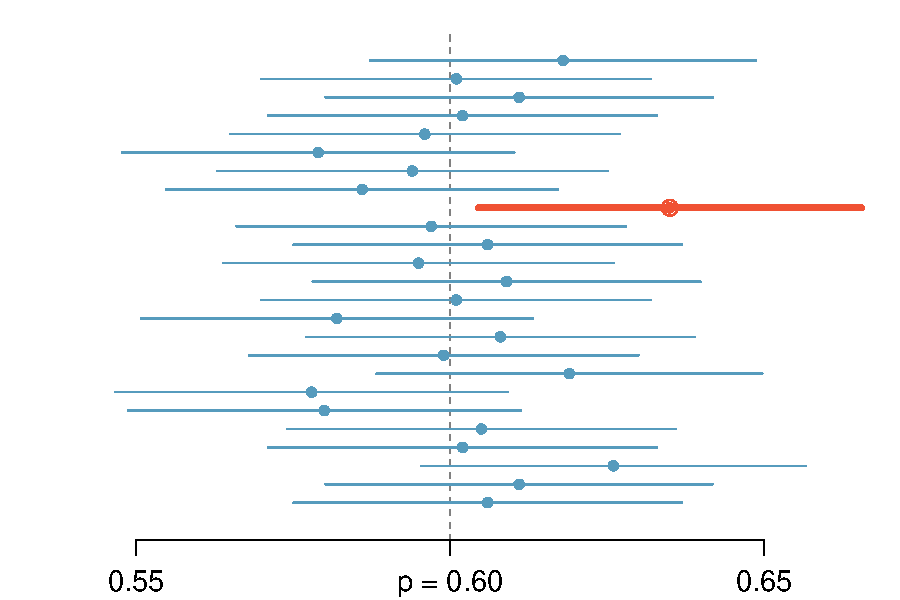
\includegraphics[width=0.75\textwidth]{05/figures/95PercentConfidenceInterval/95PercentConfidenceIntervalPHat}
   \caption{Twenty-five samples of size $n=1000$ were taken from a population where $p = 0.60$. For each sample, a 95\% confidence interval was created to try to capture the population proportion, $p = 0.60$. Only~1 of these~25 intervals did not capture the true proportion.}
   \label{95PercentConfidenceIntervalPHat}
\end{figure}

\begin{exercise}
In Figure~\ref{95PercentConfidenceIntervalPHat}, one interval does not contain 0.60. Does this imply that the population proportion cannot actually be 0.60? \footnote{Just as some observations occur more than 1.96 standard deviations from the mean, some point estimates will be more than 1.96 standard errors from the parameter. A confidence interval only provides a plausible range of values for a parameter. While we might say other values are implausible based on the data, this does not mean they are impossible.}
\end{exercise}

\begin{example}{Our owner had taken a simple random sample of mature pine trees on her property and found that 35 of 250 had damage from pine beetles. Construct a 95\% confidence interval for the true proportion of mature pine trees on her property that have pine beetle damage}\label{95CIForPineBeetleExampleForPropertyOwner}
The point estimate in this case is the sample proportion: $\hat{p} = \frac{35}{250} = 0.14$.

We can compute the standard error using the sample proportion $\hat{p} = 0.14$ and the sample size $n = 250$:
\begin{align*}
SE
	= \sqrt{\frac{p(1-p)}{n}}
	\approx \sqrt{\frac{\hat{p}(1-\hat{p})}{n}}
	= \sqrt{\frac{0.14 \times 0.86}{250}}
	= 0.022
\end{align*}
Since both $n\hat{p} = 35 \geq 10$ and $n(1-\hat{p}) = 215 \geq 10$, we can use the normal approximation for the sample proportion and calculate a 95\% confidence interval:
\begin{align*}
\text{point estimate}\ &\pm\ 1.96\times SE \\
0.14 &\pm\ 1.96\times 0.022 \\
(0.097,& 0.183)
\end{align*}
That is, we are 95\% confident that between 9.7\% and 18.3\% of the trees on the owner's property have mountain pine beetle damage.
\end{example}

When using a confidence interval with the normal distribution in the context of a sample proportion, it is called a \term{one-proportion Z interval}.

\begin{exercise}\label{largeParkPineBeetleGPFor95CI}
Suppose a large park collects data about pine beetle damage to a simple random sample of 100 mature pine trees, and 27 trees are found to be damaged. Create a 95\% confidence interval for the fraction of mature pine trees in the park that have been damaged by beetles.\footnote{We will again use a one-proportion Z interval. We can verify $n\hat{p} \geq 10$ and $n(1-\hat{p}) \geq 10$, and since the observations are from a simple random sample, the data are independent. That is, the point estimate will be nearly normal, so our confidence interval formula will be valid. Next, compute the point estimate ($\hat{p} = 27 / 100 = 0.27$) and standard error ($SE = \sqrt{0.27 \times 0.73 / 100} = 0.044$). Finally, we can plug these values into the formula for a 95\% confidence interval:
\begin{align*}
\text{point estimate}\ &\pm\ 1.96\times SE \\
0.27 &\pm\ 1.96\times 0.044
(0.184,& 0.356)
\end{align*}
We are 95\% confident that between 18.4\% and 35.6\% of the park's mature pine trees have been damaged by mountain pine beetles.}
\end{exercise}


\subsection{Changing the confidence level}
\label{changingTheConfidenceLevelSection}

\index{confidence interval!confidence level|(}

Suppose we want to consider confidence intervals where the confidence level is somewhat higher than 95\%: perhaps we would like a confidence level of 99\%. Think back to the analogy about trying to catch a fish: if we want to be more sure that we will catch the fish, we should use a wider net. To create a 99\% confidence level, we must also widen our 95\% interval. On the other hand, if we want an interval with lower confidence, such as 90\%, we could make our original 95\% interval slightly slimmer.

The 95\% confidence interval structure provides guidance in how to make intervals with new confidence levels. Below is a general 95\% confidence interval for a point estimate that comes from a nearly normal distribution:
\begin{eqnarray}
\text{point estimate}\ \pm\ 1.96\times SE
\end{eqnarray}
There are three components to this interval: the point estimate, ``1.96'', and the standard error. The choice of $1.96\times SE$ was based on the normal model for capturing the central 95\% of the distribution. That is, the choice of 1.96 corresponds to a 95\% confidence level.

\begin{exercise} \label{leadInForMakingA99PercentCIExercise}
If $X$ is a normally distributed random variable, how often will $X$ be within 2.58 standard deviations of the mean?\footnote{This is equivalent to asking how often the $Z$ score will be larger than -2.58 but less than 2.58. (For a picture, see Figure~\ref{choosingZForCI}.) To determine this probability, look up -2.58 and 2.58 in the normal probability table (0.0049 and 0.9951). Thus, there is a $0.9951-0.0049 \approx 0.99$ probability that the unobserved random variable $X$ will be within 2.58 standard deviations of $\mu$.}
\end{exercise}

To create a 99\% confidence interval, change 1.96 in the 95\% confidence interval formula to be $2.58$. Guided Practice~\ref{leadInForMakingA99PercentCIExercise} highlights that 99\% of the time a normal random variable will be within 2.58 standard deviations of the mean. This approach -- using the Z scores in the normal model to compute confidence levels -- is appropriate when $\hat{p}$ is associated with a normal distribution with mean $p$ and standard error $SE_{\hat{p}}$. Thus, the formula for a 99\% confidence interval is
\begin{eqnarray}
\hat{p}\ \pm\ 2.58\times SE_{\hat{p}}
\label{99PercCIForPHat}
\end{eqnarray}

\begin{figure}
\centering
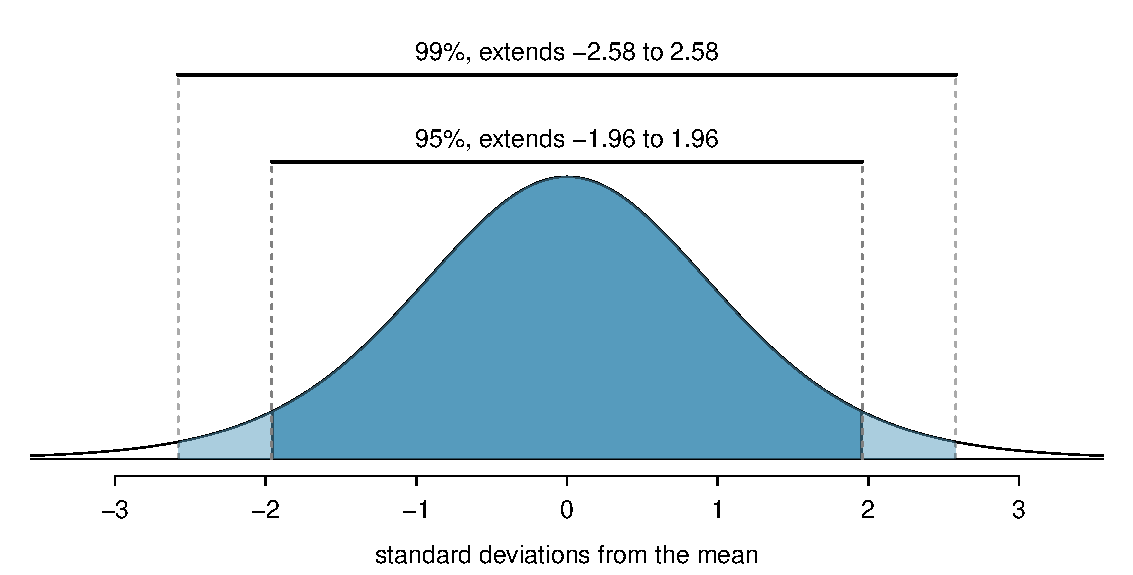
\includegraphics[width=\textwidth]{05/figures/choosingZForCI/choosingZForCI}
\caption{The area between -$z^{\star}$ and $z^{\star}$ increases as $|z^{\star}|$ becomes larger. If the confidence level is 99\%, we choose $z^{\star}$ such that 99\% of the normal curve is between -$z^{\star}$ and $z^{\star}$, which corresponds to 0.5\% in the lower tail and 0.5\% in the upper tail: $z^{\star}=2.58$.}
\label{choosingZForCI}
\index{confidence interval!confidence level|)}
\end{figure}

The normal approximation is crucial to the precision of these confidence intervals. Section~\ref{} provides a more detailed discussion about when the normal model can safely be applied. When the normal model is not a good fit, we will use alternative distributions that better characterize the sampling distribution.

\begin{termBox}{\tBoxTitle{Conditions for $\hat{p}$ being nearly normal and $SE$ being accurate\label{terBoxOfCondForXBarBeingNearlyNormalAndSEBeingAccurate}}
Important conditions to help ensure the sampling distribution of $\hat{p}$ is nearly normal and the estimate of SE sufficiently accurate:
\begin{itemize}
\setlength{\itemsep}{0mm}
\item The sample observations are independent.
\item The sample size is sufficiently large: $np \geq 10$ and $n(1-p) \geq 10$. For confidence intervals, we check $n\hat{p} \geq 10$ and $n(1-\hat{p}) \geq 10$.
\end{itemize}}
\end{termBox}

Verifying independence is often the most difficult of the conditions to check, and the way to check for independence varies from one situation to another. However, we can provide simple rules for the most common scenarios.

\begin{tipBox}{\tipBoxTitle{How to verify sample observations are independent}
Observations in a simple random sample consisting of less than 10\% of the population are independent.}
\end{tipBox}

\begin{caution}
{Independence for random processes and experiments}
{If a sample is from a random process or experiment, it is important to verify the observations from the process or subjects in the experiment are nearly independent and maintain their independence throughout the process or experiment. Usually subjects are considered independent if they undergo random assignment in an experiment.}
\end{caution}

% WARNING !!!!
% EOCE 4.9 (as of OS2) references the results of this exercise
\Comment{Must adjust EOCE 4.9.}

\begin{exercise} \label{find99CIForRun10AgeExercise}\label{find99CIForPropOfPineBeetleDamagedTrees}
Create a 99\% confidence interval for the fraction of mature pine trees on the property owner's land that are damaged by pine beetles. The point estimate is $\hat{p} = 0.14$ and the standard error is $SE_{\hat{p}} = 0.022$.\footnote{We again use a on-proportion confidence interval. The observations are independent (said to be from a simple random sample) and both $n\hat{p} = 35 \geq 10$ and $n(1-\hat{p}) = 215 \geq 10$, so the normal approximation is reasonable. Apply the 99\% confidence interval formula: $\hat{p}\ \pm\ 2.58 \times  SE_{\hat{p}} \rightarrow (0.083, 0.197)$. We are 95\% confident that between 8.3\% and 19.7\% of the trees on the owner's property have pine beetle damage.}
\end{exercise}

\begin{termBox}{\tBoxTitle{Confidence interval for any confidence level}
If the point estimate follows the normal model with standard error $SE$, then a confidence interval for the population parameter is
\begin{eqnarray*}
\text{point estimate}\ \pm\ z^{\star} SE
\end{eqnarray*}
where $z^{\star}$ corresponds to the confidence level selected.}
\end{termBox}

Figure~\ref{choosingZForCI} provides a picture of how to identify $z^{\star}$ based on a confidence level. We select $z^{\star}$ so that the area between -$z^{\star}$ and $z^{\star}$ in the normal model corresponds to the confidence level.

\begin{termBox}{\tBoxTitle{Margin of error}
\label{marginOfErrorTermBox}In a confidence interval, $z^{\star}\times SE$ is called the \term{margin of error}.}
\end{termBox}

\begin{exercise}\label{find90CIForPropOfPineBeetleDamagedTrees}
%\label{find90CIForRun10AgeExercise}
Use the data in Guided Practice~\ref{find99CIForPropOfPineBeetleDamagedTrees} to create a 90\% confidence interval for the proportion of mature pine trees damaged by beetles on the owner's property.\footnote{We again are using a one-proportion Z interval, and the conditions have already been checked. Before constructing the confidence interval, we first find $z^{\star}$ such that 90\% of the distribution falls between -$z^{\star}$ and $z^{\star}$ in the standard normal model with $\mu=0$ and $\sigma=1$. We can look up -$z^{\star}$ in the normal probability table by looking for a lower tail of 5\% (the other 5\% is in the upper tail): $z^{\star} = 1.65$. The 90\% confidence interval can then be computed as $\hat{p}\ \pm\ 1.65\times SE_{\hat{p}} \to (0.104, 0.176)$. We are 95\% confident that between 10.4\% and 17.6\% of the trees on the owner's property have pine beetle damage.}
\end{exercise}

\index{confidence interval!interpretation|)}


\subsection{Using confidence intervals: a stepwise approach}

Follow these six steps when carrying out any confidence interval problem. \Comment{Tweaked term box below, specifically the title, intro, item 3, and item 6.}

\begin{termBox}{\tBoxTitle[]{Steps for using confidence intervals (AP exam tip)}
The AP exam is scored in a standardized way, so to ensure you get all the points for a problem, make sure you complete each of the following steps.
\begin{enumerate}
\setlength{\itemsep}{0mm}
\item State the \textbf{name of the CI} being used.
\item Verify \textbf{conditions} to ensure the standard error estimate is reasonable and the point estimate is nearly normal and unbiased.
\item \textbf{Plug in the numbers} and write the interval in the form\vspace{-1mm}
\begin{align*}
\text{point estimate } \pm \text{ critical value}\times \text{SE of estimate}
\end{align*}\vspace{-1mm}% Leave this comment (formatting)
So far, the \term{critical value} has taken the form $z^\star$.
\item Evaluate the CI and \textbf{write in the form (\underline{\ \ \ \ \ }, \underline{\ \ \ \ \ })}.
\item \textbf{Interpret the interval}:  ``We are [XX]\% confident that the true [describe the parameter in context] falls between [identify the upper and lower endpoints of the calculated interval].
\item State your \textbf{conclusion} to the original question. (Sometimes, as in the case of the examples in this section, no conclusion is necessary.)
\end{enumerate}}
\end{termBox}

\index{confidence interval|)}


%__________________
\section{Hypothesis testing}
\label{hypothesisTesting}

\index{hypothesis testing|(}

The property owner with a potential pine beetle problem on their property might consider if what is happening on her property is normal. Suppose the local government has indicated that if a property owner finds that their property has more than 12\% of their mature trees to be damaged by pine beetles, they recommend that the owner explore options for mitigating further damage.

In addition to considering mountain pine beetles in this section, we consider an important topic to many students: success on an AP Statistics exam. In 2014, about 59.4\% of students earned a score of 3 or more on the AP Statistics exam.\footnote{\href{http://openintro.org/redirect.php?go=apstat2014_data&referrer=aps0}{http://www.totalregistration.net/index.php?option=com\_content\&view=article\&id=494\&Itemid=118}} However, school may suspect their students might be performing differently than schools nationally. We will consider examples for such schools throughout this section. % investigate this topic in Section~\ref{pValue}.

\begin{example}{An administer at a large private high school is curious whether their students who take AP Statistics outperform students at other schools on the exam. When she looks for data about the performance of the students at her school, she finds that 53 students took the exam and 39 earned a 3 or~higher. Create a 90\% confidence interval for the pass rate (3 or higher on the AP Statistics exam) for students at her high school.}
We will use a one-proportion Z interval. While the students are not a simple random sample, we will assume independence, e.g. that they did not influence each other's performance (which may or may not be reasonable depending on how the class was conducted). The $n\hat{p} = 12 \geq 10$ and $n(1-\hat{p}) = 39 \geq 10$ guidelines are satisfied, so we can treat $\hat{p}$ as nearly normal for a confidence interval, which is constructed as follows:
\begin{align*}
\text{point estimate} &\pm \text{critical value} \times \text{SE} \\
\hat{p} &\pm z^\star \times SE \\
0.736 &\pm 1.65 \times \sqrt{\frac{0.736 \times 0.264}{53}} \\
(0.636,& 0.836)
\end{align*}
We are 90\% confident that the true AP Statistics pass rate for students at this high school is between 63.6\% and 83.6\%.
\end{example}


\subsection{Hypothesis testing framework}

The property owner we have considered found that 14\% of the mature pine trees on her property have been damaged by pine beetles. While this is above the 12\% guideline set by the local government, she wonders whether the 14\% might just be explained by chance. Perhaps only 12\% of the trees on her property are damaged and she just got 14\% in her sample by chance. She wants to be sure, since if she does need to seek help, it will be expensive. We can simplify her perspective into two competing \termsub{hypotheses}{hypothesis}:
\begin{itemize}
\setlength{\itemsep}{0mm}
\item[$H_0$:] 12\% of the trees on her property have been damaged by pine beetles, in line with what is deemed acceptable.
\item[$H_A$:] More than 12\% of the trees on her property have been damaged, and she should seek help, which may be expensive.
\end{itemize}
We call $H_0$\marginpar[\raggedright\vspace{6mm}

$H_0$\\\footnotesize null hypothesis\vspace{3mm}\\\normalsize $H_A$\\\footnotesize alternative\\ hypothesis]{\raggedright\vspace{6mm}

$H_0$\\\footnotesize null hypothesis\vspace{3mm}\\\normalsize $H_A$\\\footnotesize alternative\\ hypothesis} the null hypothesis and $H_A$ the alternative hypothesis.

\begin{termBox}{\tBoxTitle{Null and alternative hypotheses}
{\small The \term{null hypothesis ($H_0$)} often represents either a skeptical perspective or a claim to be tested. The \term{alternative hypothesis ($H_A$)} represents an alternative claim under consideration and is often represented by a range of possible parameter values.}}
\end{termBox}

The null hypothesis often represents a skeptical position or a perspective of no difference. The alternative hypothesis often represents a new perspective, such as the possibility that there has been a change.

\begin{tipBox}{\tipBoxTitle{Hypothesis testing framework}
The skeptic will not reject the null hypothesis ($H_0$), unless the evidence in favor of the alternative hypothesis ($H_A$) is so strong that she rejects $H_0$ in favor of $H_A$.}
\end{tipBox}

The hypothesis testing framework is a very general tool, and we often use it without a second thought. If a person makes a somewhat unbelievable claim, we are initially skeptical. However, if there is sufficient evidence that supports the claim, we set aside our skepticism and reject the null hypothesis in favor of the alternative. The hallmarks of hypothesis testing are also found in the US court system.

\begin{exercise} \label{hypTestCourtExample}
A US court considers two possible claims about a defendant: she is either innocent or guilty. If we set these claims up in a hypothesis framework, which would be the null hypothesis and which the alternative?\footnote{The jury considers whether the evidence is so convincing (strong) that there is no reasonable doubt regarding the person's guilt; in such a case, the jury rejects innocence (the null hypothesis) and concludes the defendant is guilty (alternative hypothesis).}
\end{exercise}

Jurors examine the evidence to see whether it convincingly shows a defendant is guilty. Even if the jurors leave unconvinced of guilt beyond a reasonable doubt, this does not mean they believe the defendant is innocent. This is also the case with hypothesis testing: \emph{even if we fail to reject the null hypothesis, we typically do not accept the null hypothesis as true}. Failing to find strong evidence for the alternative hypothesis is not equivalent to accepting the null hypothesis as true.

In the example with our property owner, the null hypothesis represents the view that there is no difference in the proportion of trees with damage on her property than the 12\% rate deemed acceptable. In this case, the alternative hypothesis represents something more interesting, and more expensive: more than 12\% of the trees on her property are damaged, and she should seek services to help treat trees on her property. These hypotheses can be described in mathematical notation using the unknown population proportion $p$ of trees that have been damaged:
\begin{itemize}
\setlength{\itemsep}{0mm}
\item[$H_0$:] $p = 0.12$
\item[$H_A$:] $p > 0.12$
\end{itemize}
Using this mathematical notation, the hypotheses can now be evaluated using statistical tools. We call 0.12 the \term{null value} since it represents the value of the parameter if the null hypothesis is true. Usually we denote the null value with a subscript zero: $p_0 = 0.12$.


\subsection{Testing hypotheses using confidence intervals}
\label{utilizingOurCI}

We can start the evaluation of the hypothesis setup by comparing $\hat{p}$ to the null value, $p_0 = 0.12$. This estimate suggests our property owner might have a pine beetle problem. However, to evaluate whether this provides strong evidence that there is such a problem, we must consider the uncertainty associated with $\hat{p}$.

We discussed in Section~\ref{} that there is fluctuation from one sample proportion to another, and it is very unlikely that the sample proportion will be exactly equal to the population parameter (the true population proportion). That is, we should not expect $\hat{p}$ to exactly equal $p_0 = 0.12$, even if the true proportion is 0.12. Given that $\hat{p} = 0.14$, it might still be possible that the actual proportion of trees damaged by pine beetles is 0.12. The difference between $\hat{p}$ and 0.12 could be due to \emph{sampling variation}, i.e. the variability associated with the point estimate when we take a random sample.

\begin{example}{Confidence intervals were introduced in Section~\ref{} as a way to find a range of plausible values for the population proportion. Use a 90\% confidence interval for the proportion of trees damaged by pine beetles on the owner's property to evaluate the hypothesis test.}
We constructed a 90\% confidence interval for the proportion of trees damaged by pine beetles as
\begin{eqnarray*}
(0.104, 0.176)
\end{eqnarray*}
Because the null value, $p_0 = 0.12$, falls in the range of plausible values, we cannot say the null hypothesis is implausible. That is, we failed to reject the null hypothesis,~$H_0$.

In the case of our property owner, while the 14\% estimate is concerning, it does not strong evidence that there is a pine beetle problem on her property.(In Section~\ref{}, we'll explain why we used a 90\% confidence interval.)
\end{example}

\begin{tipBox}{\tipBoxTitle{Double negatives can sometimes be used in statistics}
In many statistical explanations, we use double negatives. For instance, we might say that the null hypothesis is \emph{not implausible} or we \emph{failed to reject} the null hypothesis. Double negatives are used to communicate that while we are not rejecting a position, we are also not saying it is correct.}
\end{tipBox}

\begin{example}{The administer we encountered in Example~\ref{} was originally curious whether the students who take the AP Statistics exam at their school outperform students nationally, where 59.4\% earn a 3 or higher. Construct hypotheses and use her 90\% confidence interval of $(0.636, 0.836)$ to evaluate the hypotheses.}
We can summarize the administrators viewpoint as follows:
\begin{itemize}
\item[$H_0$:] $p = 0.594$. The administrator should be skeptical that her school is any different, so the null hypothesis is that her school's performance is on par with schools nationally.
\item[$H_A$:] $p > 0.594$. Because the administrator is interested in seeing whether her school is doing better, the alternative hypothesis is that the proportion who score a 3 or higher is above the national average.
\end{itemize}
Because the null value, $p_0 = 0.594$, falls outside of the range of plausible values, we reject the null hypothesis,~$H_0$. That is, the administrator can conclude that the students at her school outperformed schools nationally.
\end{example}


\subsection{Decision errors and Power}
\index{hypothesis testing!decision errors|(}

Hypothesis tests are not flawless. Just think of the court system: innocent people are sometimes wrongly convicted and the guilty sometimes walk free. Similarly, we can make a wrong decision in statistical hypothesis tests. However, the difference is that we have the tools necessary to quantify how often we make such errors.

There are two competing hypotheses: the null and the alternative. In a hypothesis test, we make a statement about which one might be true, but we might choose incorrectly. There are four possible scenarios in a hypothesis test, which are summarized in Table~\ref{fourHTScenarios}.

\begin{table}[ht]
\centering
\begin{tabular}{l l c c}
& & \multicolumn{2}{c}{\textbf{Test conclusion}} \\
  \cline{3-4}
\vspace{-3.7mm} \\
& & do not reject $H_0$ &  reject $H_0$ in favor of $H_A$ \\
  \cline{2-4}
\vspace{-3.7mm} \\
& $H_0$ true & okay &  Type~1 Error \\
\raisebox{1.5ex}{\textbf{Truth}} & $H_A$ true & Type 2 Error & okay \\
  \cline{2-4}
\end{tabular}
\caption{Four different scenarios for hypothesis tests.}
\label{fourHTScenarios}
\end{table}

\begin{termBox}{\tBoxTitle{Type I and Type II Errors}
A~\term{Type~1 Error} is rejecting the null hypothesis when $H_0$ is actually true. A~\term{Type~2 Error} is failing to reject the null hypothesis when the alternative is actually true.}
\end{termBox}

\begin{exercise} \label{whatAreTheErrorTypesInUSCourts}
In a US court, the defendant is either innocent ($H_0$) or  guilty ($H_A$). What does a Type~1 Error represent in this context? What does a Type 2 Error represent? Table~\ref{fourHTScenarios} may be useful.\footnote{If the court makes a Type~1 Error, this means the defendant is innocent ($H_0$ true) but wrongly convicted. A Type 2 Error means the court failed to reject $H_0$ (i.e. failed to convict the person) when she was in fact guilty ($H_A$ true).}
\end{exercise}

\begin{exercise} \label{howToReduceType1ErrorsInUSCourts}
How could we reduce the Type~1 Error rate in US courts? What influence would this have on the Type 2 Error rate?\footnote{To lower the Type~1 Error rate, we might raise our standard for conviction from ``beyond a reasonable doubt'' to ``beyond a conceivable doubt'' so fewer people would be wrongly convicted. However, this would also make it more difficult to convict the people who are actually guilty, so we would make more Type~2 Errors.}
\end{exercise}

\begin{exercise} \label{howToReduceType2ErrorsInUSCourts}
How could we reduce the Type~2 Error rate in US courts? What influence would this have on the Type~1 Error rate?\footnote{To lower the Type~2 Error rate, we want to convict more guilty people. We could lower the standards for conviction from ``beyond a reasonable doubt'' to ``beyond a little doubt''. Lowering the bar for guilt will also result in more wrongful convictions, raising the Type~1 Error rate.}
\end{exercise}

\index{hypothesis testing!decision errors|)}

Guided Practice~\ref{whatAreTheErrorTypesInUSCourts}-\ref{howToReduceType2ErrorsInUSCourts} provide an important lesson: if we reduce how often we make one type of error, we generally make more of the other type.

Hypothesis testing is built around rejecting or failing to reject the null hypothesis. That is, we do not reject $H_0$ unless we have strong evidence. But what precisely does \emph{strong evidence} mean? As a general rule of thumb, for those cases where the null hypothesis is actually true, we do not want to incorrectly reject $H_0$ more than 5\% of the time. This corresponds to a \term{significance level}\index{hypothesis testing!significance level} of 0.05. We often write the significance level using $\alpha$\marginpar[\raggedright\vspace{-4mm}

$\alpha$\\\footnotesize significance\\level of a\\hypothesis test]{\raggedright\vspace{-4mm}

$\alpha$\\\footnotesize significance\\level of a\\hypothesis test} (the Greek letter \emph{alpha}\index{Greek!alpha@alpha ($\alpha$)}): $\alpha = 0.05$. We discuss the appropriateness of different significance levels in Section~\ref{significanceLevel}.

A \term{Type~1 Error} is rejecting the null hypothesis when $H_0$ is actually true. A \term{Type~2 Error} is failing to reject the null hypothesis when the alternative is actually true.

If we use a 95\% confidence interval to test a hypothesis where the null hypothesis is true, we will make an error whenever the point estimate is at least 1.96 standard errors away from the population parameter. This happens about 5\% of the time (2.5\% in each tail). Similarly, using a 99\% confidence interval to evaluate a hypothesis is equivalent to a significance level of $\alpha = 0.01$.

A confidence interval is, in one sense, simplistic in the world of hypothesis tests. Consider the following two scenarios:
\begin{itemize}
\setlength{\itemsep}{0mm}
\item The null value (the parameter value under the null hypothesis) is in a 95\% confidence interval but just barely, so we would not reject $H_0$. However, we might like to somehow say, quantitatively, that it was a close decision.
\item The null value is very far outside of the interval, so we reject $H_0$. However, we want to communicate that, not only did we reject the null hypothesis, but it wasn't even close. Such a case is depicted in Figure~\ref{whyWeWantPValue_prop}.
\end{itemize}
In Section~\ref{pValue}, we introduce a tool called the \emph{p-value} that will be helpful in these cases. The p-value method also extends to hypothesis tests where confidence intervals cannot be easily constructed or applied.

\begin{figure}[hht]
\centering
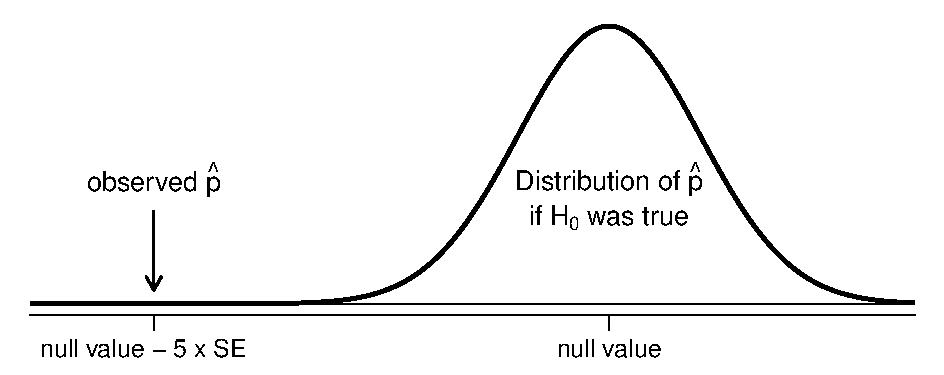
\includegraphics[width=0.75\textwidth]{05/figures/whyWeWantPValue/whyWeWantPValue_prop}
\caption{It would be helpful to quantify the strength of the evidence against the null hypothesis. In this case, the evidence is extremely strong.}
\label{whyWeWantPValue_prop}
\end{figure}


\subsection{Formal testing using p-values}
\label{pValue}

\index{hypothesis testing!p-value|(}

The p-value is a way of quantifying the strength of the evidence against the null hypothesis and in favor of the alternative. Formally the \emph{p-value} is a conditional probability.

\begin{termBox}{\tBoxTitle{p-value}
The \term{p-value}\index{hypothesis testing!p-value|textbf} is the probability of observing data at least as favorable to the alternative hypothesis as our current data set, if the null hypothesis is true. We typically use a summary statistic of the data, in this chapter the sample mean, to help compute the p-value and evaluate the hypotheses.}
\end{termBox}

% \Comment{This example was removed in favor of breaking it down over a couple of pages so key ideas could be more easily highlighted.}
%\begin{example}{Redo the hypothesis test for the property owner who has a possible pine beetle problem, but this time use p-values.}
%We will use what is called a \term{one-proportion hypothesis test}. The hypotheses are unchanged from before and are shown below, and we will use a significance level of $\alpha = 0.05$.
%\begin{itemize}
%\setlength{\itemsep}{0mm}
%\item[$H_0$:] $p = 0.12$
%\item[$H_A$:] $p > 0.12$
%\end{itemize}
%For confidence intervals, we have used $\hat{p}$ in place of $p$ to check conditions ($np \geq 10$ and $n(1-p) \geq 10$) and also to compute the standard error ($SE = \sqrt{p (1 - p) / n}$). However, the standard approach in a one-proportion hypothesis test is to use the null value for these calculations. In this case, we use $p_0 = 0.12$:
%\begin{align*}
%np_0 = 30 &\geq 10
%	& n(1-p_0) = 220 &\geq 10
%	& SE &= \sqrt{\frac{p_0 (1 - p_0)}{n}}
%		= \sqrt{\frac{0.12 \times 0.88}{250}}
%		= 0.021
%\end{align*}
%Because $\hat{p}$ is nearly normal, we 
%\end{example}

We revisit the hypothesis test for the property owner who has a possible pine beetle problem, but this time we formally run the \term{one-proportion hypothesis test} using the p-value approach. The hypotheses are unchanged from before:
\begin{itemize}
\setlength{\itemsep}{0mm}
\item[$H_0$:] $p = 0.12$
\item[$H_A$:] $p > 0.12$
\end{itemize}
Using $p > 0.12$ as the alternative is an example of a \term{one-sided} hypothesis test. In this investigation, there is no apparent interest in learning whether the proportion is less than 0.12.\footnote{This is entirely based on the interests of the owner. Had she been only interested in the opposite case -- showing that trees on her property had a pine beetle damage rate \emph{below} 0.12, then our setup would have set the alternative as $p < 0.12$.} In many future examples, we will use a \term{two-sided} hypothesis where we looked for any clear difference, greater than or less than the null value.

Always use a two-sided test unless it was made clear prior to data collection that the test should be one-sided. Switching a two-sided test to a one-sided test after observing the data is dangerous because it can inflate the Type~1 Error rate. 

\begin{tipBox}{\tipBoxTitle{One-sided and two-sided tests}
If the researchers are only interested in showing an increase or a decrease, but not both, use a one-sided test. If the researchers would be interested in any difference from the null value -- an increase or decrease -- then the test should be two-sided.\vspace{0.5mm}}
\end{tipBox}

\begin{tipBox}{\tipBoxTitle{Always write the null hypothesis as an equality}
We will find it most useful if we always list the null hypothesis as an equality (e.g. $p = 0.12$) while the alternative always uses an inequality (e.g. $p \neq 0.12$, $p > 0.12$, or $p < 0.12$).}
\end{tipBox}

Before we can use a normal model for the sample proportion or compute the standard error of the sample proportion, we must verify conditions. For confidence intervals, we used $\hat{p}$ in place of $p$ to check the minimum expected count conditions ($np \geq 10$ and $n(1-p) \geq 10$) and also to compute the standard error ($SE = \sqrt{p (1 - p) / n}$). However, the standard approach in a one-proportion hypothesis test is to use the null value for these calculations. In this case, we use $p_0 = 0.12$:
\begin{align*}
np_0
	&= 30
	\geq 10
	\qquad\qquad
	n(1-p_0)
		= 220
		\geq 10 \\
SE &= \sqrt{\frac{p_0 (1 - p_0)}{n}}
	= \sqrt{\frac{0.12 \times 0.88}{250}}
	= 0.021
\end{align*}
In this case, the normal model still seems reasonable.

\begin{termBox}{\tBoxTitle{Conditions and standard error in a one-proportion hypothesis test}
In a one-proportion hypothesis test, we always check conditions and compute the standard error using the null value, $p_0$. \emph{This is a critical detail for being both statistically correct and for getting full credit on the AP exam.}}
\end{termBox}

We'll evaluate the property owner's hypothesis test using a significance level of $\alpha = 0.05$. We want to consider the data under the scenario that the null hypothesis is true. In this case, the sample proportion is from a nearly normal distribution with mean 0.12 and standard deviation of about 0.021. Such a distribution is shown in Figure~\ref{pValueOneSidedPropertyOwnerWithTheBeetleProblem}.

\begin{figure}[hht]
   \centering
   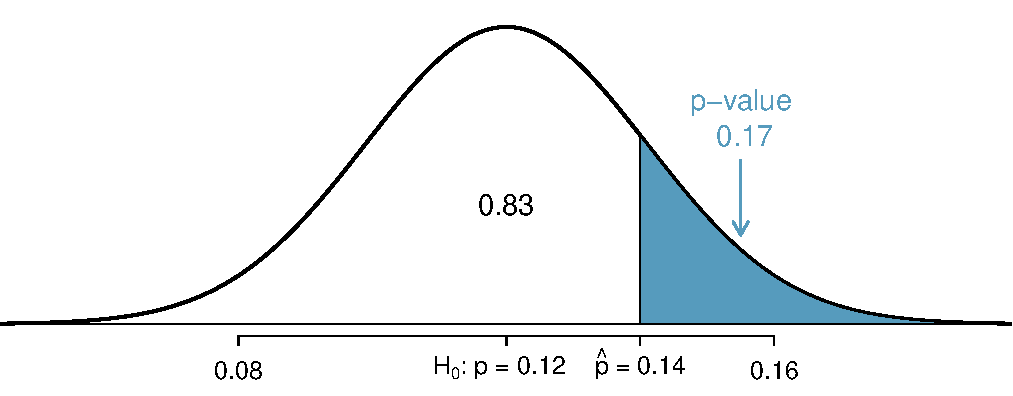
\includegraphics[width=0.73\textwidth]{05/figures/PineBeetle/pValueOneSidedPropertyOwnerWithTheBeetleProblem}
   \caption{If the null hypothesis is true, then the sample proportion $\hat{p}$ came from this nearly normal distribution. The right tail describes the probability of observing such a large sample proportion if the null hypothesis is true.}
\label{pValueOneSidedPropertyOwnerWithTheBeetleProblem}
\end{figure}

The shaded tail in Figure~\ref{pValueOneSidedPropertyOwnerWithTheBeetleProblem} represents the chance of observing such a large sample proportion, conditional on the null hypothesis being true. That is, the shaded tail represents the p-value. We shade all proportions larger than our sample proportion, $\hat{p} = 0.14$, because they are more favorable to the alternative hypothesis than the observed mean.

We compute the p-value by finding the tail area of this normal distribution, which we learned to do in Section~\ref{normalDist}. First compute the Z score of the sample proportion, $\hat{p} = 0.14$:
\begin{eqnarray*}
Z = \frac{\bar{x} - \text{null value}}{SE_{\bar{x}}} = \frac{0.14 - 0.12}{0.021} = 0.95
\end{eqnarray*}
Here, Z is our \term{test statistic}. Using the normal probability table, the unshaded area is found to be 0.83. Thus the shaded area is $1 - 0.83 = 0.17$. \emph{If the null hypothesis is true, the probability of observing such a large sample proportion for a sample of 250 pine trees is 0.17.}\index{p-value!interpretation example}

We evaluate the hypotheses by comparing the p-value to the significance level. Because the p-value is greater than the significance level (p-value $= 0.17 > 0.05 =\alpha$), we do not reject the null hypothesis. That is, if the true proportion is 0.12, what we have observed is not so unusual. The property owner does not have strong evidence that the proportion of trees on her property that have been damaged by pine beetles is different than 0.12.

\begin{termBox}{\tBoxTitle{p-value as a tool in hypothesis testing}
The p-value quantifies how strongly the data favor $H_A$ over $H_0$. A small p-value (usually $<0.05$) corresponds to sufficient evidence to reject $H_0$ in favor of $H_A$.}
\index{hypothesis testing!p-value|)}
\end{termBox}

\begin{tipBox}{\tipBoxTitle{Draw a picture or use a calculator to find the p-value}
It is useful to draw a picture of the distribution of $\hat{p}$ as though $H_0$ was true (i.e. $p$ equals the null value), and shade the region(s) of sample proportions that are at least as favorable to the alternative hypothesis. These shaded regions represent the p-value.\vspace{3mm}

Alternatively or additionally, is also reasonable to carefully use a calculator or statistical software to calculate the p-value.}
\end{tipBox}

The ideas below review the process of evaluating hypothesis tests with p-values:
\begin{itemize}
\setlength{\itemsep}{0mm}
\item The null hypothesis represents a skeptic's position or a position of no difference. We reject this position only if the evidence strongly favors $H_A$.
\item A small p-value means that if the null hypothesis is true, there is a low probability of seeing a point estimate at least as extreme as the one we saw. We interpret this as strong evidence in favor of the alternative.
\item We reject the null hypothesis if the p-value is smaller than the significance level, $\alpha$, which is usually 0.05. Otherwise, we fail to reject $H_0$.
\item We should always state the conclusion of the hypothesis test in plain language so non-statisticians can also understand the results.
\end{itemize}

The p-value is constructed in such a way that we can directly compare it to the significance level ($\alpha$) to determine whether or not to reject $H_0$. This method ensures that the Type~1 Error rate does not exceed the significance level standard.

\begin{figure}[ht]
\centering
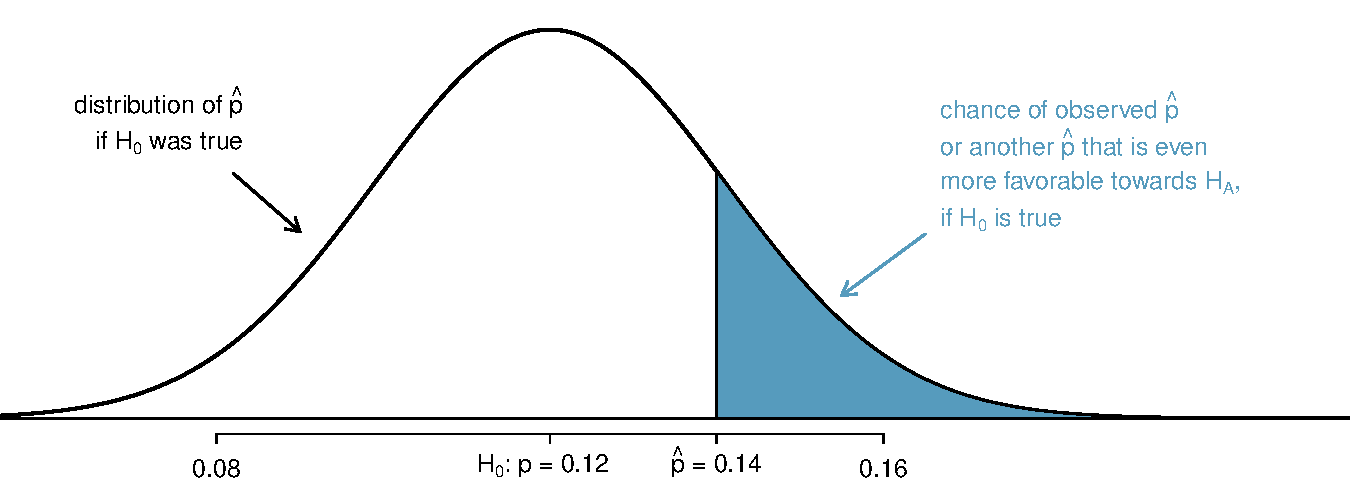
\includegraphics[width=0.9\textwidth]{05/figures/PineBeetle/pValueOneSidedBeetleStudyExplained}
\caption{To identify the p-value, the distribution of the sample proportion is considered as if the null hypothesis was true. Then the p-value is defined and computed as the probability of the observed $\hat{p}$ or an $\hat{p}$ even more favorable to $H_A$ under this distribution.}
\label{pValueOneSidedSleepStudyExplained}
\end{figure}

\begin{exercise}
If the null hypothesis is true, how often should the p-value be less than 0.05?\footnote{About 5\% of the time. If the null hypothesis is true, then the data only has a 5\% chance of being in the 5\% of data most favorable to $H_A$.}
\end{exercise}

\begin{exercise}
Suppose we had used a significance level of 0.10 in the property owner case study. Would the evidence have been strong enough to reject the null hypothesis? The p-value was 0.17.~\footnote{We reject the null hypothesis whenever $p$-$value < \alpha$. Since the p-value is still larger than $\alpha$, we would still \emph{not} reject the null hypothesis if $\alpha = 0.10$.}
\end{exercise}

\begin{termBox}{\tBoxTitle{What's so special about 0.05?}
We often use a threshold of 0.05 to determine whether a result is statistically significant. But why 0.05? Maybe we should use a bigger number, or maybe a smaller number. If you're a little puzzled, that probably means you're reading with a critical eye -- good job! We've made a video to help clarify \emph{why 0.05}:
\begin{center}
\href{http://www.openintro.org/why05}{www.openintro.org/why05}
\end{center}
Of course, ometimes it's also a good idea to deviate from the standard. We'll discuss when to choose a threshold different than 0.05 in Section~\ref{}.\vspace{0.5mm}}
\end{termBox}


\subsection{Two-sided hypothesis testing with p-values}
\label{twoSidedTestsWithPValues}

Consider the school administrator who was interested in checking whether her school was outperforming the national average. Of course, it is also possible the school falls below the average, but this wasn't really considered!

Such a possibility wasn't considered in the earlier hypothesis test. This may have seemed natural since the data pointed in the directions of interest to the administrator. However, there are two dangers if we ignore possibilities that disagree with our data or that conflict with our worldview:
\begin{enumerate}
\item Framing an alternative hypothesis simply to match the direction that the data point will generally inflate the Type 1 Error rate. After all the work we've done (and will continue to do) to rigorously control the error rates in hypothesis tests, careless construction of the alternative hypotheses can disrupt that hard work. We'll explore this topic further in Section~\ref{InflatingType1ErrorRate}.
\item If we only use alternative hypotheses that agree with our worldview, then we're going to be subjecting ourselves to \term{confirmation bias}, which means we look for data that supports our ideas. That's not very scientific, and we can do better!
\end{enumerate}
The previous hypotheses we've seen are called \term{one-sided hypothesis tests} because they only explored one direction of possibilities. Such hypotheses are appropriate when we are exclusively interested in the single direction. Usually we want to consider all possibilities. In the school administrator's example, she certainly would have been interested if the school was underperforming, so a \term{two-sided hypothesis test} would have been more appropriate.

\begin{example}{Conduct a two-sided hypothesis test for the school administrator. Her school had 53 students who took the AP Statistics test in 2014, and 39 of them passed. She would like to know if her school is \emph{different} than the national average, 59.4\%.}
We will again use a one-proportion hypothesis test with a two-sided hypothesis setup:
\begin{itemize}
\item[$H_0$:] $p = 0.594$. The administrator should be skeptical that her school is any different, so the null hypothesis is that her school's performance is on par with schools nationally.
\item[$H_A$:] $p \neq 0.594$. Because the administrator is actually interested in any \emph{difference}, we use $\neq$ instead of $>$ or $<$.
\end{itemize}
We will use a significance level of $\alpha = 0.05$. As we learned in Section~\ref{}, we should check the test's $np \geq 10$ and $n(1-p) \geq 10$ conditions and compute the standard error using the null value:
\begin{align*}
np_0
	&= 53 \times 0.594
	= 31.5
	\geq 10
	\qquad\qquad
	n(1-p_0)
		53 \times 0.406
		= 21.5
		\geq 10 \\
SE &= \sqrt{\frac{p_0 (1 - p_0)}{n}}
	= \sqrt{\frac{0.594 \times 0.406}{53}}
	= 0.0675
\end{align*}
In this case, the normal model still seems reasonable. The standard error is also a little larger than when we estimated it using $\hat{p}$ instead of $p_0$.

We will compute a Z score of the sample proportion as our test statistic:
\begin{align*}
Z = \frac{\hat{p} - p_0}{SE}
	= \frac{0.736 - 0.594}{0.0675}
	= 2.10
\end{align*}
Figure~\ref{ap_stat_admin_2_sided_test} highlights the p-value for this hypothesis test. We use both the left \emph{and} right tails since data in either direction from $p_0 = 0.594$ would support the alternative hypothesis.

The area of either tail can be identified ($\approx0.018$), then we can double it to get the area of both tails:
\begin{align*}
\text{p-value}
	= 2 \times \text{(one-tail area)}
	= 2 \times 0.018
	= 0.036
\end{align*}
Because the p-value (0.036) is less than $\alpha = 0.05$, we reject the null hypothesis. Our result is unchanged from before, and we can conclude the administrator's school \term{statistically significantly} outperformed the national average.
\end{example}

\begin{figure}[ht]
\centering
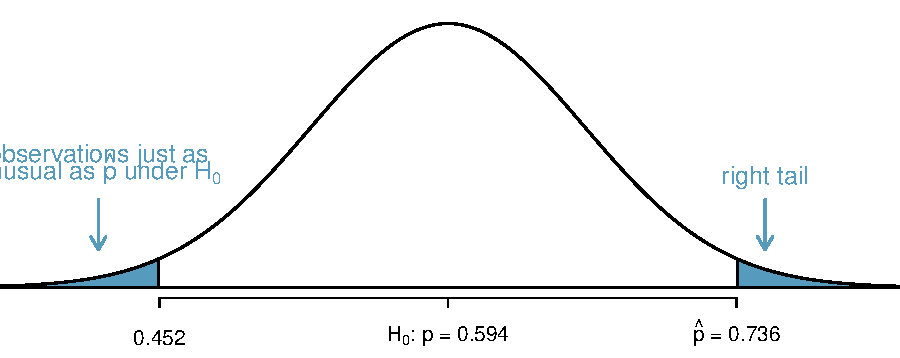
\includegraphics[width=0.95\textwidth]{05/figures/ap_stat_admin/ap_stat_admin_2_sided_test}
\caption{In a two-sided test, the p-value comprises \emph{both} the original tail and also the opposite tail, since any observations in these ranges provide stronger evidence against the null hypotheses than the observed data.}
\label{ap_stat_admin_2_sided_test}
\end{figure}

In one-sided tests, we shade the single tail in the direction of the alternative hypothesis. In a two-sided test, \emph{we shade both tails} since evidence in either direction is favorable to $H_A$.

\begin{example}{It is never okay to change two-sided tests to one-sided tests after observing the data. In this example we explore the consequences of ignoring this advice. Using $\alpha=0.05$, we show that freely switching from two-sided tests to one-sided tests will cause us to make twice as many Type~1 Errors as intended.} \label{swappingHypAfterDataDoublesType1ErrorRate}
Suppose the sample proportion was larger than the null value, $p_0$ (e.g. $p_0$ would represent~0.594 if $H_0$:~$p = 0.594$). Then if we can flip to a one-sided test, we would use $H_A$: $p > p_0$. Now if we obtain any $\hat{p}$ with a test statistic (Z score) greater than 1.65, we would reject $H_0$. If the null hypothesis is true, we incorrectly reject the null hypothesis about 5\% of the time when the sample proportion is above the null value, as shown in Figure~\ref{type1ErrorDoublingExampleFigureProp}.

Suppose the sample proportion was smaller than the null value. Then if we change to a one-sided test, we would use $H_A$: $p < p_0$. If $\hat{p}$ had a test statistic smaller than -1.65, we would reject $H_0$. If the null hypothesis is true, then we would observe such a case about 5\% of the time.

By examining these two scenarios, we can determine that we will make a Type~1 Error $5\%+5\%=10\%$ of the time if we are allowed to swap to the ``best'' one-sided test for the data. This is twice the error rate we prescribed with our significance level: $\alpha=0.05$ (!).

\begin{figure}
   \centering
   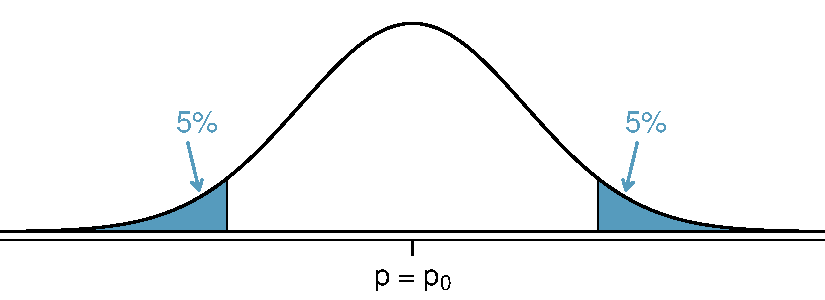
\includegraphics[width=0.7\textwidth]{05/figures/type1ErrorDoublingExampleFigure/type1ErrorDoublingExampleFigure_prop}
   \caption{The shaded regions represent areas where we would reject $H_0$ under the bad practices considered in Example~\ref{swappingHypAfterDataDoublesType1ErrorRate} when $\alpha = 0.05$.}
   \label{type1ErrorDoublingExampleFigure}
\end{figure}

\end{example}

\begin{caution}{One-sided hypotheses are allowed only \emph{before} seeing data}
{After observing data, it is tempting to turn a two-sided test into a one-sided test. Avoid this temptation. Hypotheses must be set up \emph{before} observing the data or only if there is interest in a one-sided result.}
\end{caution}


\subsection{Choosing a significance level}
\label{significanceLevel}

\index{hypothesis testing!significance level|(}
\index{significance level|(}

Choosing a significance level for a test is important in many contexts, and the traditional level is 0.05. However, it is often helpful to adjust the significance level based on the application. We may select a level that is smaller or larger than 0.05 depending on the consequences of any conclusions reached from the test.

If making a Type~1 Error is dangerous or especially costly, we should choose a small significance level (e.g. 0.01). Under this scenario we want to be very cautious about rejecting the null hypothesis, so we demand very strong evidence favoring $H_A$ before we would reject $H_0$.

If a Type 2 Error is relatively more dangerous or much more costly than a Type~1 Error, then we should choose a higher significance level (e.g. 0.10). Here we want to be cautious about failing to reject $H_0$ when the null is actually false.

\begin{tipBox}{\tipBoxTitle[]{Significance levels should reflect consequences of errors}
The significance level selected for a test should reflect the consequences associated with Type~1 and Type~2 Errors.}
\end{tipBox}

\begin{example}{A car manufacturer is considering a higher quality but more expensive supplier for window parts in its vehicles. They sample a number of parts from their current supplier and also parts from the new supplier. They decide that if the high quality parts will last more than 12\% longer, it makes financial sense to switch to this more expensive supplier. Is there good reason to modify the significance level in such a hypothesis test?}
The null hypothesis is that the more expensive parts last no more than 12\% longer while the alternative is that they do last more than 12\% longer. This decision is just one of the many regular factors that have a marginal impact on the car and company. A significance level of 0.05 seems reasonable since neither a Type~1 or Type 2 error should be dangerous or (relatively) much more expensive.
\end{example}

\begin{example}{The same car manufacturer is considering a slightly more expensive supplier for parts related to safety, not windows. If the durability of these safety components is shown to be better than the current supplier, they will switch manufacturers. Is there good reason to modify the significance level in such an evaluation?}
The null hypothesis would be that the suppliers' parts are equally reliable. Because safety is involved, the car company should be eager to switch to the slightly more expensive manufacturer (reject $H_0$) even if the evidence of increased safety is only moderately strong. A slightly larger significance level, such as $\alpha=0.10$, might be appropriate.
\end{example}

\begin{exercise}
A part inside of a machine is very expensive to replace. However, the machine usually functions properly even if this part is broken, so the part is replaced only if we are extremely certain it is broken based on a series of measurements. Identify appropriate hypotheses for this test (in plain language) and suggest an appropriate significance level.\footnote{Here the null hypothesis is that the part is not broken, and the alternative is that it is broken. If we don't have sufficient evidence to reject $H_0$, we would not replace the part. It sounds like failing to fix the part if it is broken ($H_0$ false, $H_A$ true) is not very problematic, and replacing the part is expensive. Thus, we should require very strong evidence against $H_0$ before we replace the part. Choose a small significance level, such as $\alpha=0.01$.}
\end{exercise}

\index{significance level|)}
\index{hypothesis testing!significance level|)}



\subsection{Formal hypothesis testing: a stepwise approach\vspace{-3mm}}

\Comment{Moved all content into the term box, adjusted the intro in term box, and adjusted items 6 and 7.}

\begin{termBox}{\tBoxTitle{Carrying out a formal test of hypothesis}
Follow these seven steps when carrying out a hypothesis test. This is both good practice and also be useful for the AP exam.
\begin{enumerate}
\setlength{\itemsep}{0mm}
\item State the \textbf{name of the test} being used.
\item First write the \textbf{hypotheses} in plain language, then set them up in mathematical notation.
\item Identify the \textbf{significance level} $\alpha$.
\item Verify \textbf{conditions} to ensure the standard error estimate is reasonable and the point estimate is nearly normal and unbiased.
\item Calculate the \textbf{test statistic}, often Z, using an appropriate point estimate of the parameter of interest and its standard error.\vspace{-1.5mm}
\begin{align*}
\text{test statistic} = \frac{\text{point estimate} - \text{null value}}{\text{SE of estimate}}
\end{align*}
\item Find the \textbf{p-value}, compare it to $\alpha$, and state whether to reject or not reject the null hypothesis.
\item Write your \textbf{conclusion}.
\end{enumerate}}
\end{termBox}

\index{hypothesis testing|)}



%__________________
\section{Does it make sense?}
\subsection{When to retreat}
\label{whenToRetreat}

Statistical tools rely on conditions. When the conditions are not met, these tools are unreliable and drawing conclusions from them is treacherous. The conditions for these tools typically come in two forms.
\begin{itemize}
\setlength{\itemsep}{0mm}
\item \textbf{The individual observations must be independent.} A random sample from less than 10\% of the population ensures the observations are independent. In experiments, we generally require that subjects are randomized into groups. If independence fails, then advanced techniques must be used, and in some such cases, inference may not be possible.
\item \textbf{Other conditions focus on sample size and skew.} For example, if the sample size is too small, the skew too strong, or extreme outliers are present, then the normal model for the sample mean will fail.
\end{itemize}
Verification of conditions for statistical tools is always necessary. Whenever conditions are not satisfied for a statistical technique, there are three options. The first is to learn new methods that are appropriate for the data. The second route is to consult a statistician.\footnote{If you work at a university, then there may be campus consulting services to assist you. Alternatively, there are many private consulting firms that are also available for hire.} The third route is to ignore the failure of conditions. This last option effectively invalidates any analysis and may discredit novel and interesting findings.

Finally, we caution that there may be no inference tools helpful when considering data that include unknown biases, such as convenience samples. For this reason, there are books, courses, and researchers devoted to the techniques of sampling and experimental design. See Sections~\ref{overviewOfDataCollectionPrinciples}-\ref{experimentsSection} for basic principles of data collection.


\subsection{Statistical significance versus practical significance}

When the sample size becomes larger, point estimates become more precise and any real differences in the mean and null value become easier to detect and recognize. Even a very small difference would likely be detected if we took a large enough sample. Sometimes researchers will take such large samples that even the slightest difference is detected. While we still say that difference is \term{statistically significant}, it might not be \term{practically significant}.

Statistically significant differences are sometimes so minor that they are not practically relevant. This is especially important to research: if we conduct a study, we want to focus on finding a meaningful result. We don't want to spend lots of money finding results that hold no practical value.

The role of a statistician in conducting a study often includes planning the size of the study. The statistician might first consult experts or scientific literature to learn what would be the smallest meaningful difference from the null value. She also would obtain some reasonable estimate for the standard deviation. With these important pieces of information, she would choose a sufficiently large sample size so that the power for the meaningful difference is perhaps 80\% or 90\%. While larger sample sizes may still be used, she might advise against using them in some cases, especially in sensitive areas of research.


\subsection{Statistical power of a hypothesis test}

When the alternative hypothesis is true, the probability of \underline{not} making a Type~2 Error is called \term{power}. It is common for researchers to perform a \hiddenterm{power analysis} to ensure their study collects enough data to detect the effects they anticipate finding. As you might imagine, if the effect they care about is small or subtle, then if the effect is real, the researchers will need to collect a large sample size in order to have a good chance of detecting the effect. However, if they are interested in large effect, they need not collect as much data.

The Type 2 Error rate $\beta$ and the magnitude of the error for a point estimate are controlled by the sample size. Real differences from the null value, even large ones, may be difficult to detect with small samples. If we take a very large sample, we might find a statistically significant difference but the magnitude might be so small that it is of no practical value.




%__________________
\section{Inference for other estimators (special topic)}

The sample proportion is not the only point estimate for which the sampling distribution is nearly normal. For example, the sampling distribution of the sample mean closely resembles the normal distribution when the sample size is sufficiently large. In this section, we introduce a number of examples where the normal approximation is reasonable for the point estimate. Chapters~\ref{inferenceForCategoricalData} and~\ref{inferenceForNumericalData} will revisit each of the point estimates you see in this section along with other new statistics.

We make an important assumption about each point estimate encountered in this section: the estimate is unbiased. A point estimate is \term{unbiased} if the sampling distribution of the estimate is centered at the parameter it estimates. That is, an unbiased estimate does not naturally over or underestimate the parameter. Rather, it tends to provide a ``good'' estimate. The sample proportion is an example of an unbiased point estimate, as are each of the examples we introduce in this section.

\Comment{Verify this content didn't get cut.} Finally, we will discuss the general case where a point estimate may follow some distribution other than the normal distribution. We also provide guidance about how to handle scenarios where the statistical techniques you are familiar with are insufficient for the problem at hand.


\subsection{Confidence intervals for nearly normal point estimates}

\index{confidence interval!using normal model|(}

In Section~\ref{} we used the point estimate $\hat{p}$ with a standard error $SE_{\hat{p}}$ to create a 95\% confidence interval for the population mean:
\begin{align*}
\hat{p}\ \pm\ 1.96 \times SE_{\hat{p}}
\end{align*}
We constructed this interval by noting that the sample proportion is within 1.96 standard errors of the actual proportion about 95\% of the time. This same logic generalizes to any unbiased point estimate that is nearly normal. We may also generalize the confidence level by using a place-holder $z^{\star}$.

\begin{termBox}{\tBoxTitle{General confidence interval for the normal sampling distribution case}\label{generalConfidenceIntervalTermBox}%
A confidence interval based on an unbiased and nearly normal point estimate is
\begin{align*}
\text{point estimate}\ \pm\ z^{\star}SE
\end{align*}
where $z^{\star}$ is selected to correspond to the confidence level, and $SE$ represents the standard error. The value $z^{\star}SE$ is called the \emph{margin of error}\index{margin of error}.}
\end{termBox}

Generally the standard error for a point estimate is estimated from the data and computed using a formula. For example, the standard error for the sample proportion is
\begin{eqnarray*}
SE_{\hat{p}} = \sqrt{\frac{p(1-p)}{n}}
\end{eqnarray*}
where we would substitute an appropriate value for $p$. In this section, we provide the computed standard error for each example and guided practice without detailing where the values came from. In future chapters, you will learn to fill in these and other details for each situation.

\begin{example}{A point estimate for the average difference in run times between men and women in the 2012 Cherry Blossom Run based on a large sample of participants is $\bar{x}_{women}-\bar{x}_{men}=14.48$ minutes. This point estimate is associated with a nearly normal distribution with standard error $SE=2.78$ minutes. What is a reasonable 95\% confidence interval for the difference in average run times?}
\label{confIntervalForDifferenceOfRunTimeBetweenGenders}
The normal approximation is said to be valid, so we apply Equation~\eqref{95PercGeneralCIInGeneralizingSection}:
\begin{eqnarray*}
\text{point estimate}\ \pm\ z^{\star} SE
	\quad\rightarrow\quad 14.48\ \pm\ 1.96\times 2.78
	\quad\rightarrow\quad (9.03, 19.93)
\end{eqnarray*}
We are 95\% confident that the men were, on average, between 9.03 and 19.93 minutes faster than women in the 2012 Cherry Blossom Run. That is, the actual average difference is plausibly between 9.03 and 19.93 minutes with 95\% confidence.
\end{example}
%library(openintro); library(xtable); data(run10); data(run10Samp); (x <- by(run10Samp$time, run10Samp$gender, mean)); diff(x); s <- by(run10Samp$time, run10Samp$gender, sd); n <- by(run10Samp$time, run10Samp$gender, length); sqrt(sum(s^2/n))


\begin{example}{Does Example~\ref{confIntervalForDifferenceOfRunTimeBetweenGenders} guarantee that if a husband and wife both ran in the race, the husband would run between 9.03 and 19.93 minutes faster than the wife?}
Our confidence interval says absolutely nothing about individual observations. It only makes a statement about a plausible range of values for the \emph{average} difference between all men and women who participated in the run.
\end{example}

\begin{exercise} \label{findZFor99PercConfLevelInFrameworkForInf}
What $z^{\star}$ would be appropriate for a 99\% confidence level? For help, see Figure~\vref{choosingZForCI}.\footnote{We seek $z^{\star}$ such that 99\% of the area under the normal curve will be between the Z scores -$z^{\star}$ and $z^{\star}$. Because the remaining 1\% is found in the tails, each tail has area 0.5\%, and we can identify -$z^{\star}$ by looking up 0.0050 in the normal probability table: $z^{\star} = 2.58$. See also Figure~\vref{choosingZForCI}.}
\end{exercise}


\subsection{Hypothesis testing for nearly normal point estimates}
\index{hypothesis testing!using normal model|(}

Just as the confidence interval method works with many other point estimates, we can generalize our hypothesis testing methods to new point estimates. Here we only consider the p-value approach, introduced in Section~\ref{pValue}, since it is the most commonly used technique and also extends to non-normal cases.

\begin{exercise} \label{fdaHypSetupForSulph}
A drug called sulphinpyrazone was under consideration for use in reducing the death rate in heart attack patients. To determine whether the drug was effective, a set of 1,475 patients were recruited into an experiment and randomly split into two groups: a control group that received a placebo and a treatment group that received the new drug. What would be an appropriate null hypothesis? And the alternative?\footnote{The skeptic's perspective is that the drug does not work at reducing deaths in heart attack patients ($H_0$), while the alternative is that the drug does work ($H_A$).}
\end{exercise}

We can formalize the hypotheses from Exercise~\ref{fdaHypSetupForSulph} by letting $p_{control}$ and $p_{treatment}$ represent the proportion of patients who died in the control and treatment groups, respectively. Then the hypotheses can be written as
\begin{eqnarray*}
&&H_0: p_{control} = p_{treatment} \quad\text{(the drug doesn't work)} \quad \\
&&H_A: p_{control} > p_{treatment} \quad\text{(the drug works)}
\end{eqnarray*}
or equivalently,
\begin{eqnarray*}
&&H_0: p_{control} - p_{treatment} = 0 \quad\text{(the drug doesn't work)} \quad \\
&&H_A: p_{control} - p_{treatment} > 0 \quad\text{(the drug works)}
\end{eqnarray*}
Strong evidence against the null hypothesis and in favor of the alternative would correspond to an observed difference in death rates,
\begin{eqnarray*}
\text{point estimate} = \hat{p}_{control} - \hat{p}_{treatment}
\end{eqnarray*}
being larger than we would expect from chance alone. This difference in sample proportions represents a point estimate that is useful in evaluating the hypotheses. 

\begin{example}{We want to evaluate the hypothesis setup from Exericse~\ref{fdaHypSetupForSulph} using data from the actual study.\footnote{Anturane Reinfarction Trial Research Group. 1980. Sulfinpyrazone in the prevention of sudden death after myocardial infarction. New England Journal of Medicine 302(5):250-256.} In the control group, 60 of 742 patients died. In the treatment group, 41 of 733 patients died. The sample difference in death rates can be summarized as
\begin{eqnarray*}
\text{point estimate} = \hat{p}_{control} - \hat{p}_{treatment} = \frac{60}{742} - \frac{41}{733} = 0.025
\end{eqnarray*}
This point estimate is nearly normal and is an unbiased estimate of the actual difference in death rates. The standard error of this sample difference is $SE = 0.013$. Evaluate the hypothesis test at a 5\% significance level: $\alpha=0.05$.}
We would like to identify the p-value to evaluate the hypotheses. If the null hypothesis is true, then the point estimate would have come from a nearly normal distribution, like the one shown in Figure~\ref{sulphStudyFindPValueUsingNormalApprox}. The distribution is centered at zero since $p_{control}-p_{treatment}=0$ under the null hypothesis. Because a large positive difference provides evidence against the null hypothesis and in favor of the alternative, the upper tail has been shaded to represent the p-value. We need not shade the lower tail since this is a one-sided test: an observation in the lower tail does not support the alternative hypothesis.

\begin{figure}[bt]
   \centering
   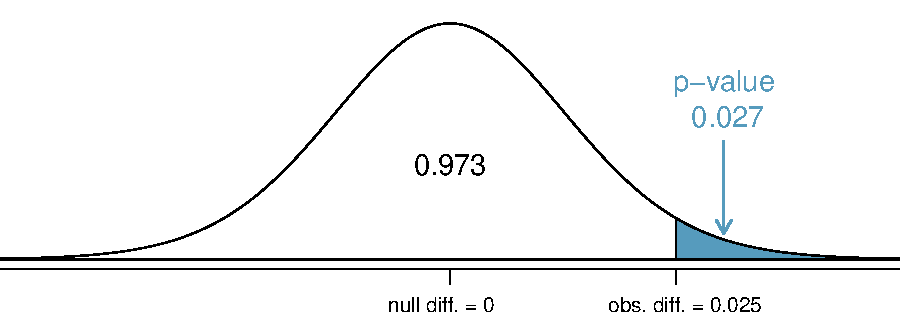
\includegraphics[height=37mm]{05/figures/sulphStudyFindPValueUsingNormalApprox/sulphStudyFindPValueUsingNormalApprox}
   \caption{The distribution of the sample difference if the null hypothesis is true.}
   \label{sulphStudyFindPValueUsingNormalApprox}
\end{figure}

The p-value can be computed using the Z score of the point estimate.
\begin{eqnarray}
Z = \frac{\text{point estimate} - \text{null value}}{SE_{\text{point estimate}}}
	= \frac{0.025 - 0}{0.013} = 1.92
\label{zScoreOfPointEstimateForSulphinpyrazoneThisIsFirstTestStatReference}
\end{eqnarray}
Examining $Z$ in the normal probability table or using a calculator, we find that the p-value (the upper tail) is about 0.027. Because the p-value is less than the significance level ($\alpha=0.05$), we say the null hypothesis is implausible. That is, we reject the null hypothesis in favor of the alternative and conclude that the drug is effective at reducing deaths in heart attack patients.
\end{example}

Just like in the one-proportion hypothesis test scenario, the Z score in Equation~(\ref{zScoreOfPointEstimateForSulphinpyrazoneThisIsFirstTestStatReference}) is called a \hiddenterm{test statistic}. In most hypothesis tests, a test statistic is a particular data summary that is especially useful for computing the p-value and evaluating the hypothesis test. In the case of point estimates that are nearly normal, the test statistic is the Z score.

\begin{termBox}{\tBoxTitle{Test statistic}
A \emph{test statistic} is a special summary statistic that is particularly useful for evaluating a hypothesis test or identifying the p-value. When a point estimate is nearly normal, we use the Z score of the point estimate as the test statistic. In later chapters we encounter situations where other test statistics are helpful.}
\index{hypothesis testing!using normal model|)}\index{test statistic}
\end{termBox}


\subsection{Non-normal point estimates}

We may apply the ideas of confidence intervals and hypothesis testing to cases where the point estimate or test statistic is not necessarily normal. There are many reasons why such a situation may arise:
\begin{itemize}
\setlength{\itemsep}{0mm}
\item the sample size is too small for the normal approximation to be valid;
\item the standard error estimate may be poor; or
\item the point estimate tends towards some distribution that is not the normal distribution.
\end{itemize}
For each case where the normal approximation is not valid, our first task is always to understand and characterize the sampling distribution of the point estimate or test statistic. Next, we can apply the general frameworks for confidence intervals and hypothesis testing to these alternative distributions.





